\documentclass[12pt,a4paper]{article}
\usepackage[utf8]{inputenc}
\usepackage{amsmath}
\usepackage{amsfonts}
\usepackage{amssymb}
\usepackage{graphicx}
\usepackage{hyperref} % For links 
\usepackage{listings} % For quoting code
\usepackage{color} %For colorful code
\usepackage{ulem} % For \sout
\author{Eric Marzec}
\title{Orca Development Guide}
\definecolor{dkgreen}{rgb}{0,0.6,0}
\definecolor{gray}{rgb}{0.5,0.5,0.5}
\definecolor{mauve}{rgb}{0.58,0,0.82}

\lstset{frame=tb,
  language=[Objective]C,
  aboveskip=3mm,
  belowskip=3mm,
  showstringspaces=false,
  columns=flexible,
  basicstyle={\small\ttfamily},
  numbers=none,
  numberstyle=\tiny\color{gray},
  keywordstyle=\color{blue},
  commentstyle=\color{dkgreen},
  stringstyle=\color{mauve},
  breaklines=true,
  breakatwhitespace=true,
  tabsize=3
  }
\begin{document}
As a pedagogical excercise this guide will show how one can add a new hardware object (in this case, the
 Toaster) to SNO+'s DAQ software, Orca. This will hopefully provide the reader with enough general
  knowledge about Orca that he/she will be able to tackle their own DAQ software related tasks without large
   amounts of pain. For this guide I assume the reader has a cursory knowledge of Objective-C and has an
    installed and working version of XCode \& Orca. 
\\
\section{Overview and Preliminaries}
Here I'll provide an overview of the process for adding and building the Toaster in Orca.
The first step to creating the Toaster will be to create the basic files that will be used to construct the Toaster. 
After that the Toaster has to be added to the Orcas catalog of hardware items,
this will make it possible to access the Toaster at run time.
The next step will be where we begin to define the actual functionality of the Toaster.
In doing so we will see how different parts of Orca communicate, how best to do networking, GUI design practices, and the myriad of details that go into accomplishing such things.
Additionally, there are a variety of Orca/XCode tid-bits that I think can be extremely towards understanding Orca that don't belong in the Toaster's narrative.
 I put these valuable nuggets of wisdom into the appendix.


Additionally this guide is far from complete or even very detailed, so for more detailed questions (but less specific answers) a good place to look is the \href{https://developer.apple.com/library/mac/navigation/}{ Apple Docs.} The Apple Docs also include a good number of getting started guides type guides, their relevance to Orca, though, can be fairly hit-or-miss.
 Nevertheless, they're a worthwhile resource for a stuck and frustrated Orca developer.
 
 Another useful resource is \href{http://orca.physics.unc.edu/Programming/Index.html}{Orca's programmers guide.}
 This guide is more complete and in some areas more detailed than that guide.
   However Orca's official guide was written by the progenitor of Orca, unlike this guide whose author(s) have much more modest expertise. 
   
 
 As a final preliminary note, the XCode working/editing environment is fairly unique and very Apple-y. 
 For the average emacs/vim die-hard this can be an unsettling change and 
 becoming familiar and comfortable with any new IDE is no mean feat. 
 Code editing can obviously be done outside of XCode, however there are some things that absolutely must be down inside of it.
 The choice is ultimately yours as to what extent you'll embrace/avoid the XCode editor.
 I'm not sure there's anything I can say in this regard that isn't at least partially subjective,
 so I'll offer no advice at all, in this matter you and you alone are the artisan of your destiny.
But should you decide to use XCode, it may be worthwhile for you to play around with the various buttons, panes,  and interfaces.
 That way when you want to do things like open a file in a new window, or a new tab, or perhaps split a window between two different files, you can do so without missing a step.

 
 
\section{Laying the Ground Work}
A good starting place is to hollow out a space in Orca where all of the Toaster's files will go.
 Almost all of the files for SNO+'s hardware are located in Orca/Objects/Custom Hardware/SNO+/.
  The best way I've found to add a new folder is to create the folder at the desired location then tell XCode about it.
So add a folder called "Toaster" in the SNO+ folder.
 Then in XCode right click on the SNO+ folder in the Project Manager tab (in the left most pane) and select "Add Files to "Orca" ".
  Then select the Toaster folder that you created, and voila, you've got a space to work.
   See, wasn't that almost as easy as it should have been.  
 \subsection{MVC}
 Before adding the actual files in which the Toaster's implementation will inhabit,
 it's worthwhile to discuss  Apple/Orca's design pattern. 
 Orca follows the Model-View-Controller (MVC) design philosophy.
 This means every hardware item that you'd like to represent should to have a model, a view, and a controller.
 Exactly what each of these do is currently unknown and we should probably figure it out.
 But I'll describe here the two schools of thought on the subject.
 The View is the interface that the users uses. 
 It's, window(s) and all the boxes, buttons, and dialogs that will be used at run-time to accept input from the user.
  Everyone pretty much agrees that this is what the View should do.
  The responsibilities of the  Controller is contentious.
  Some would argue that the controller should be a go-between for the View and the Model.
  Something that synthesizes the input from the view, and gives the resulting information to the Model.
  In this philosophy the Model is then responsible performing the changes on the actual hardware and for keeping track of that change.
  An example of this would be the user changes a threshold value in the MTC interface in the View.
   Then the Controller would read the new value from the View perhaps check if it's within some allowable bounds, and then call an appropriate function in the Model.
   The Model would then do whatever is necessary to actually change the MTC threshold, assumedly this would mean sending some information out on a socket connection.
   The Model would also store the fact that it this change was made in a variable or in a database.
   
   The alternative philosophy is that the Controller should be the one to make the change on the MTC, then
   it should tell the Model that this change was made.
   The Model then updates the variable/database.
   
   The various advantages/disadvantages are the subject of debate, but I'll not further muddy these murky waters with them. 
   The important take away is a hardware object has at least three parts, a Model, a View, and a Controller,
   and there exists a division of labor between these three parts, but together they'll define the Toaster.
   For a more professional discussion see \href{https://developer.apple.com/library/ios/documentation/General/Conceptual/CocoaEncyclopedia/Model-View-Controller/Model-View-Controller.html}
   {what Apple has to say on the subject.} 
   or if you'd prefer you can look at 
   \href{http://orca.physics.unc.edu/Programming/Code_Overview.html}
   {the official Orca take on MVC}
   
   \subsection{Adding a Model, View, and Controller}
   To add classes for the Toaster's Controller right click on the Toaster folder in the XCode Project Navigator and select new file.
  In the menu that pops up select "Cocoa Class", then in the next window give the controller some nice  self documenting name, and in "Subclass of" dropdown menu select "OrcaObjectController". 
  Also make sure the button to create a XIB file is checked.
An XIB file is the where all the GUI design is done, it will be the View for the Toaster.
With this done the Toaster folder should now have a .h and a .m file for the Controller and a .xib file for the View.
To create a Model class follow the exact same steps as before, the only difference is the Model should be a subclass of "OrcaObject" and no .XIB file needs to be created.
With this done all the basic files needed to implement the toaster exist, but before adding the toaster logic to these files, it might be best to take a detour to make sure the Toaster can be accessed at run time.
\section{Adding the Toaster to the Hardware Catalog}
Orca has a large catalog of hardware objects that can be used to build a representation of one's experiment.
So to take advantage of the Toaster's implementation in Orca, it has to be added to the catalog.
The Catalog is located in Orca/Source/Main Dialogs/Catalog.nib
\footnote{A .nib file is pretty much the same as a .xib file. 
The only difference between the two is in how XCode stores the file on disk.}.
 Almost all the hardware items for the SNO+ detector are located in Experiments and SNO Lab tab.
 The easiest way to add a new item is to simply copy and paste  a different object 
 (using CMND+c, CMND+v) and then edit the relevant properties.
  This will ensure that all properties except those specific to the Toaster are correct.

The first and foremost of such properties is the icon for the Toaster.
  If you're lazy you could just steal an icon from a different hardware item or from google but a more enterprising developer would make their own icon in MSPaint. 
  After creating your masterpiece add it to XCode by putting it in the desired directory and then right clicking in the Project Navigator and selecting "Add Files to Orca"
  From here find and select the icon.
  Make sure it ends up located in the XCode project navigator where it should be.
  Then select
  \footnote{You may notice the selecting the desired object in the XCode Interface Builder can be a labyrinth of clicking, double clicking and frustration.  
The only advice I can offer in the regard is that practice makes perfect.}
   your copied object and in the right hand properties pane, locate the image property 
   (it should be in the "Attributes Inspector" tab of the pane.)
   Here, use the drop-down menu or just type to select your icon.
   Your catalog item should now have the correct icon, doesn't it look great?
   Also in the attributes inspector you should change the title to "Toaster".
   The final property to change is the "tool tip" and can be found in the "Identity Inspector" tab.
   The tool tip must be the name of the Model for the Toaster. 
   This is what links a catalog item to the MVC hardware object.
   Take a look at a few of the other catalog items and you'll see that this is indeed the case.
  It may be worthwhile for you to spend a bit of time looking at/playing with the other properties availible in the right-hand pane.
  When you have to design your own UI's it'll be good to know what aesthetic knobs are available for turning.
   
   At this point you may think you're done with the catalog, but if you compile and run Orca you'll notice that the Toaster catalog item refuses to drag \& drop into the experiment builder area.
    The reason for this is the Model you put in the tool tip has to have at a setUpImage function in its implementation.
     The exact reason this function is needed I cannot say, but it's safe to assume that in Orca's design, somewhere between the catalog item and the actual instantiation of a hardware item, the setUpImage function gets called,
 and if it's not present the process fails.
The following is an example of a  setUpImage function (with some handy extra code commented out).

\begin{lstlisting}
   - (void) setUpImage
 {
    NSImage* img = [NSImage imageNamed:@"ToasterIconFileName"];
    //Scale image by half    
    //NSSize halfSize = [img size];
   // halfSize.height = (int)(halfSize.height / 2);
    //halfSize.width  = (int)(halfSize.width  / 2);
    //[img setSize:halfSize];
    [self setImage:img];

 }
\end{lstlisting}

With that code added to the the Model you should now be able to drag \& and drop the toaster from the catalog into a new (or existing) experiment.

\section{Basic Functionality}
\subsection{Boiler Plate}
With the catalog problem handled we're almost done handling the Orca overhead and ready to begin making the Toaster a genuine toaster.
 When you run Orca now and put the toaster in the experiment, double clicking on it doesn't bring up our (admittedly empty) toaster window.
  A few more boiler-plate functions need to be added.
  The first is a function that links your Model and your Controller, it should look something like the following.
  \begin{lstlisting}
  - (void) makeMainController
{
    [self linkToController:@"ToasterController"];
}
  \end{lstlisting}
  This function belongs in the Model's implementation.
  \\The seconds is an initialization function for the Controller that links it to the View.
\begin{lstlisting} 
  -(id)init
{
    self = [super initWithWindowNibName:@"ToasterController"];    
    [self registerNotificationObservers];

    return self;
}
\end{lstlisting}
In these two chunks of code my Controller was named ToasterController.h/m and the View was named ToasterController.xib, so although the two pieces of code both invoke an item named ToasterController, they are indeed both looking at different things.

This is all the code that is \emph{strictly} required, however there a few more pieces of code that are recommended for fully fleshed hardware object.
 These are given in Appendix \ref{App:AppendixA}
 \subsection{Clicky Buttons}
 Now that there's a window that pops up you may realize how depressingly empty that window is. 
 Let's add a button to it!
 Following the Orca fashion, all (most) GUI editing will be done with the XCode Interface Builder. This has the advantage, of being easy, intuitive, and fast,
 but the disadvantage of Orca no longer being represented by code.
 Instead it's represented by code+weird XCode magic.
 
  \begin{figure}
 \begin{center}
 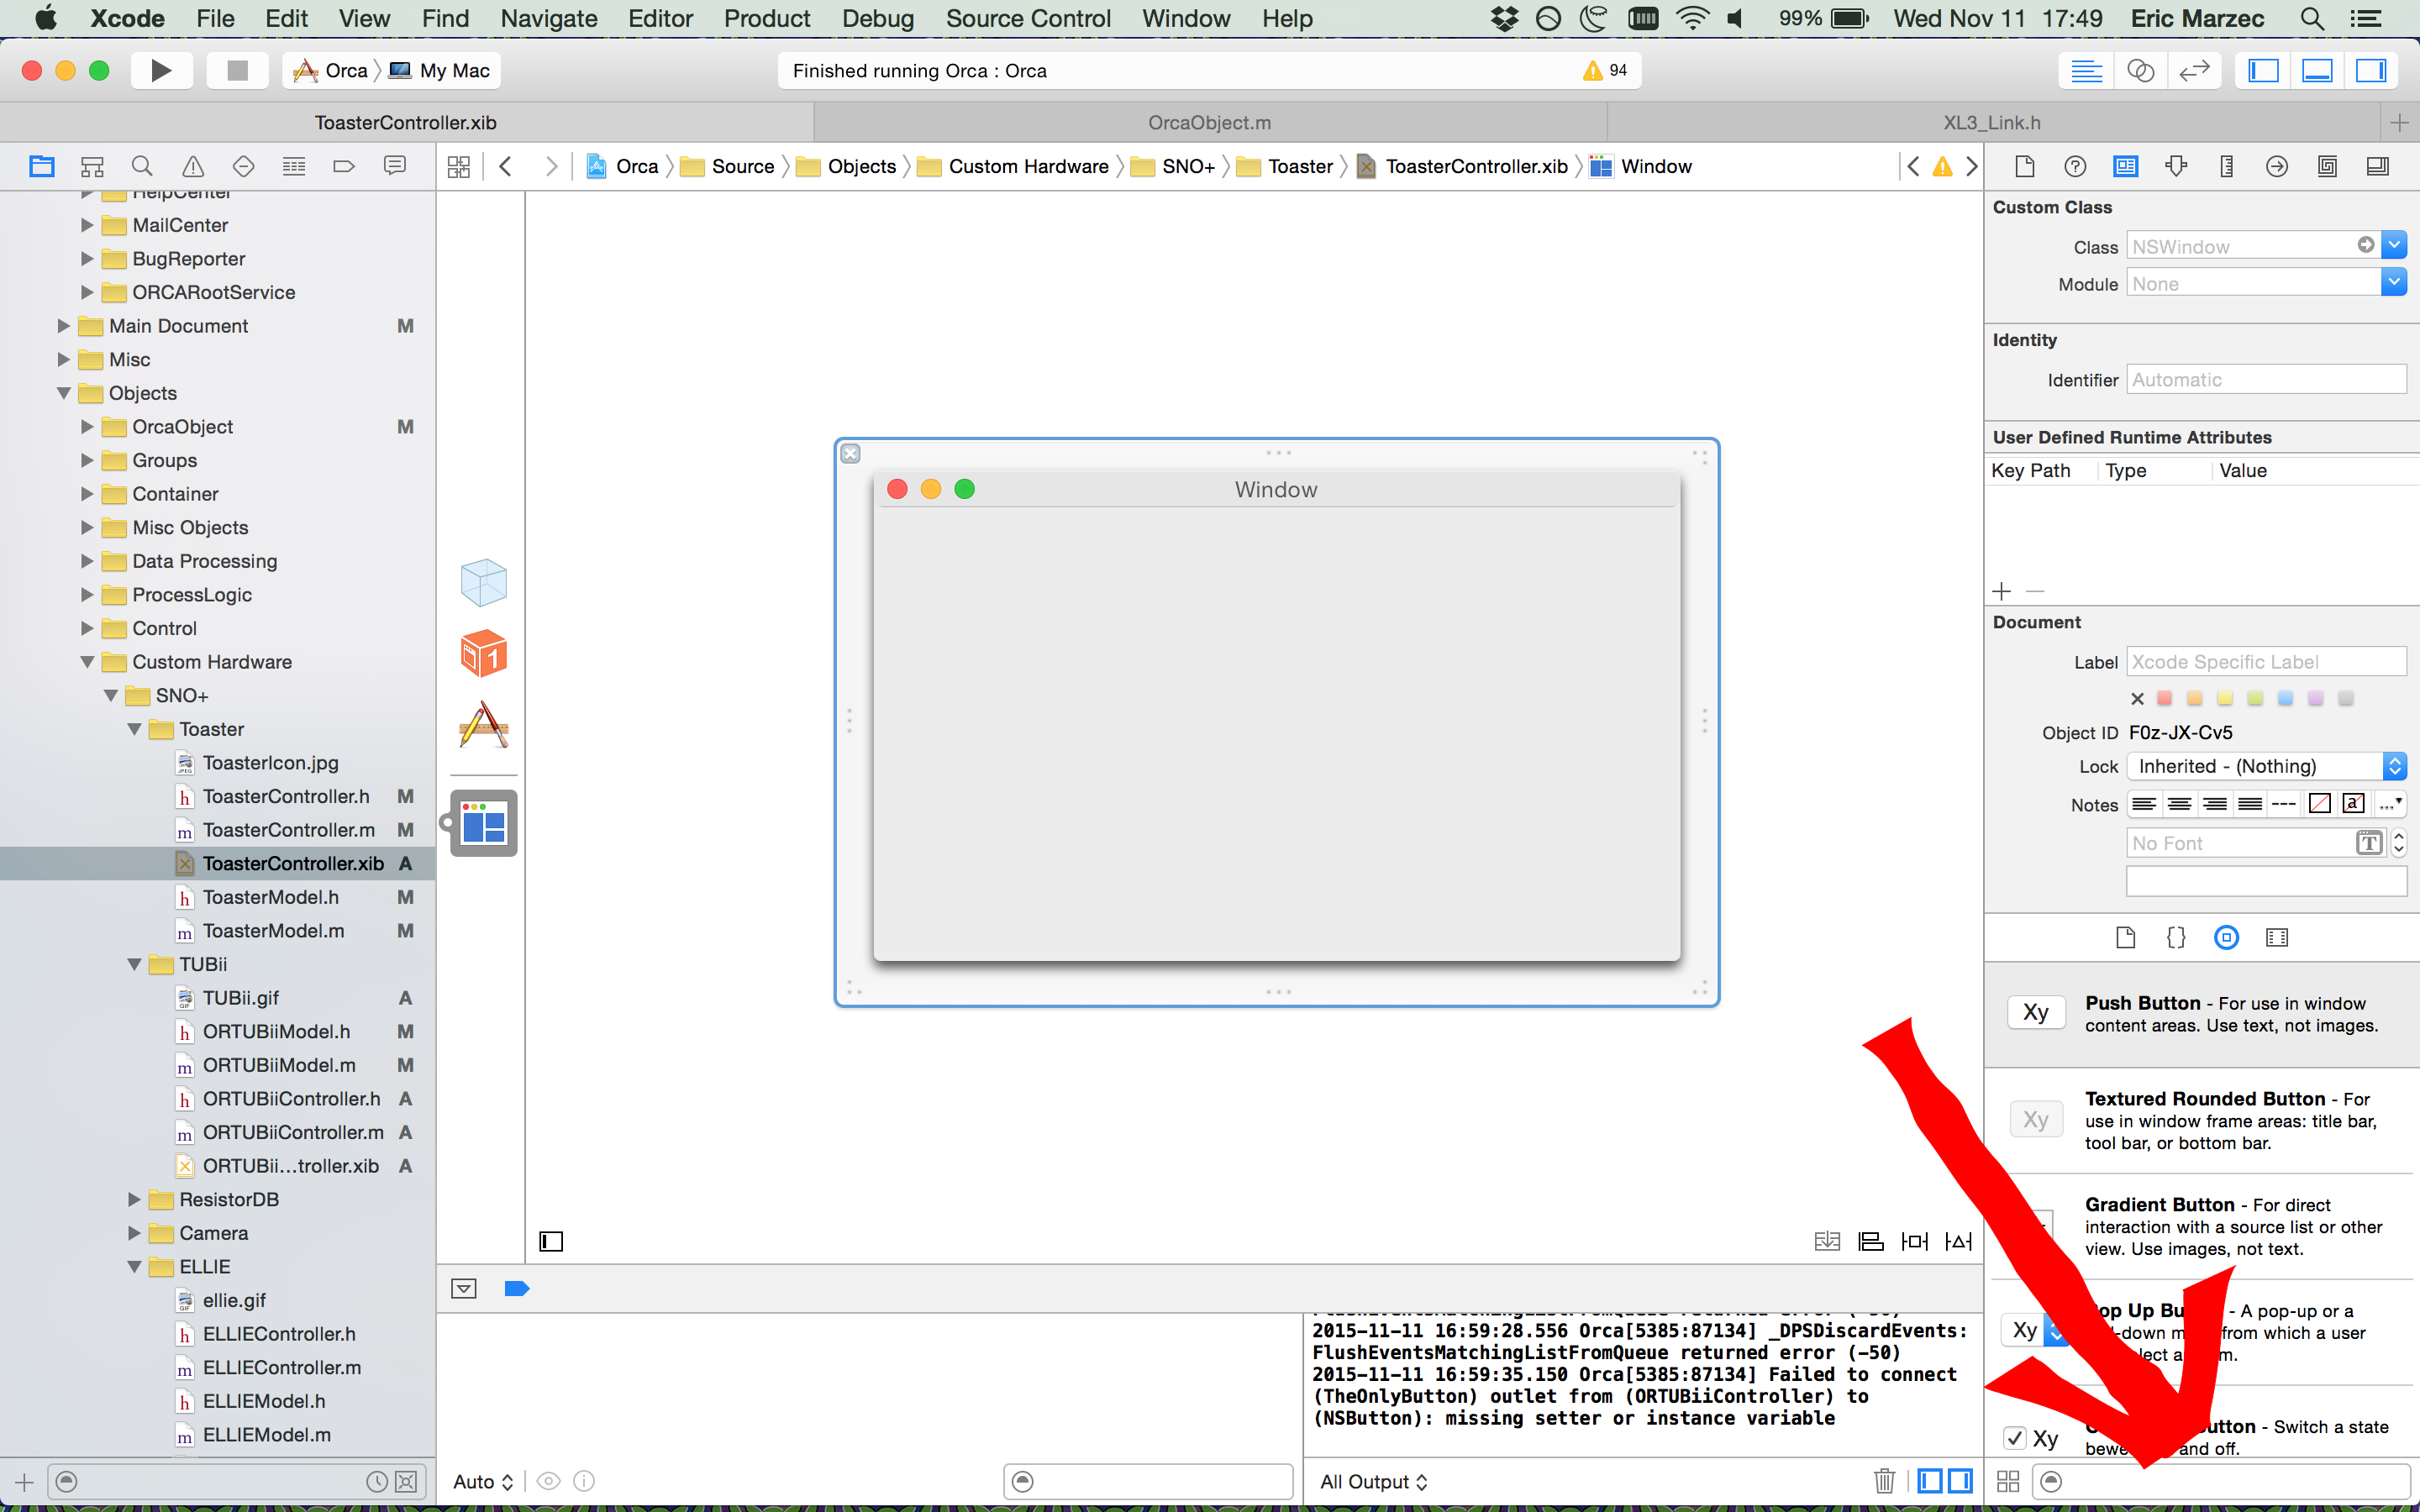
\includegraphics[width=1.0\textwidth]{GUI_Search_Dialog}
 \caption{Indicates GUI object search box location.\label{fig:GUISearchDialog}}
 \end{center}
 \end{figure}
 
 To add a button open of the Toaster's .xib file and search for "button" in the dialog indicated in Figure \ref{fig:GUISearchDialog} search for "button". Make sure the "object library" tab is selected and not one of the other searchable libraries.
 Once you've located a button that you like simply drag \& drop it to the window.
 The task now is to make that button actually do something.
 The easiest way of going about this is to split your workspace into two panes, one with the .xib file and one with the Controllers .m file.
 Then either cntrl-click and right-click the button and drag the wire that pops up into the Controller implementation.
 This should cause a dialog to appear, in that enter the name you'd like to give to the function that will be called when the button is clicked.
 For testing purposes I recommend you have the function simply write some text to NSLog, it will become more complex soon.
 \section{Making the Toaster a Toaster}
 At this point we've basically accomplished the "Hello World" of implementing a hardware item in Orca. 
 Now is where we can begin adding actual Toaster like functionality.
 There are a number of ways to begin, but to keep it simple, a simple starting point will be to have the toaster have two states, toasting or not toasting, and also have the ability to do some network communication. 
 The network communication will allow the Orca Toaster to query the actual physical Toaster, and then update its state accordingly.
\subsection{Tracking The State with Notifications} 
 Well the first and easiest thing to do is add the appropriate variable (in my case, toastEnable) to the Model and give it some getters and setters.
 It may seem reasonable to use @sythesize to make the getter/setter, but we'll want extra things to happen whenever the toaster state changes.
 So in anticipation of that it's best to write it out the long way.
 Additionally it's important to designate the toastEnable variable as a @property, so that other objects (e.g. the Controller) can access it and change it if need be.
 
  \begin{figure}[h]
 \begin{center}
 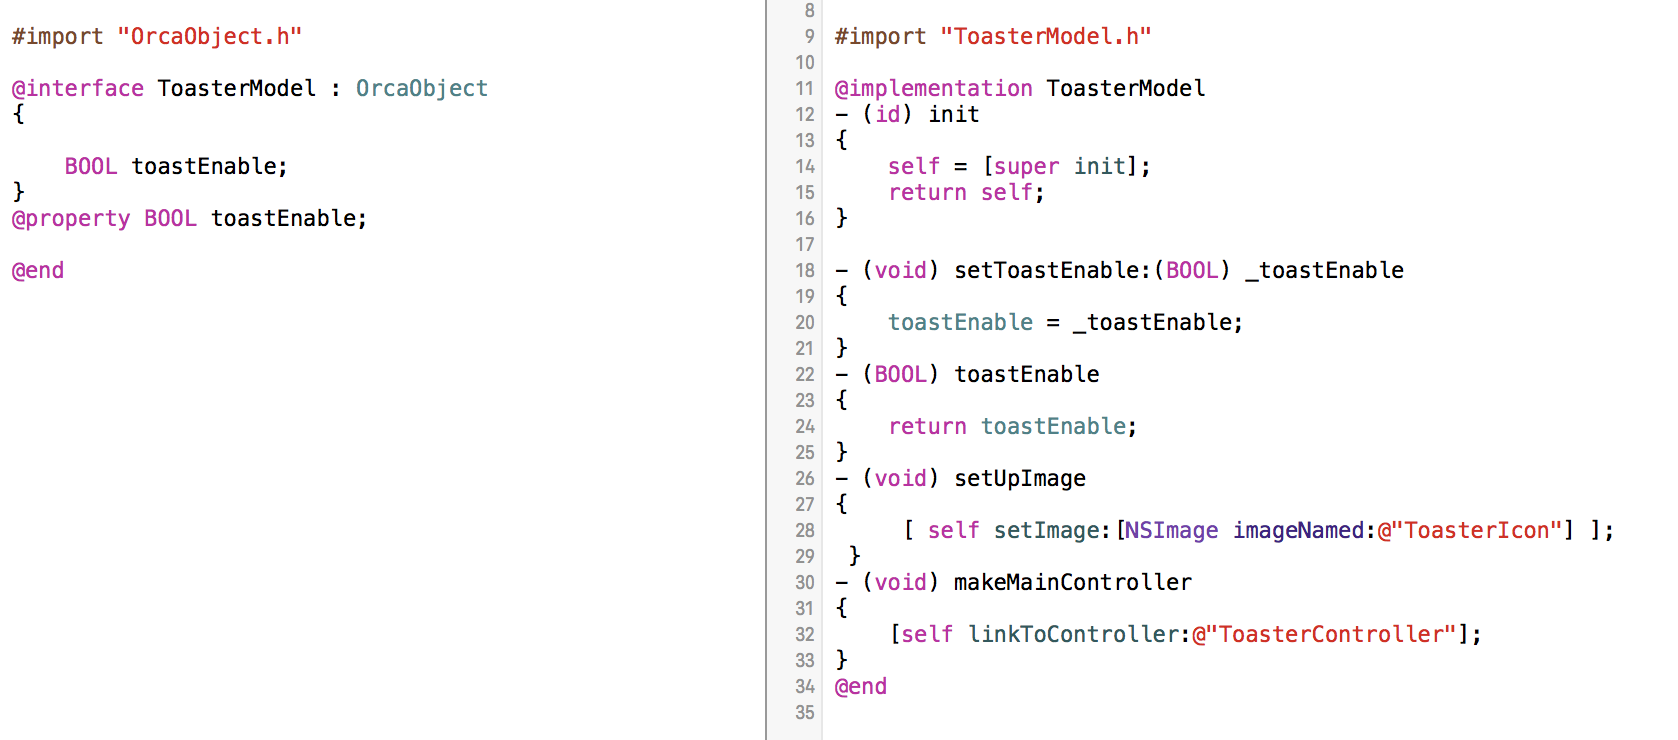
\includegraphics[width=1.0\textwidth]{ToastEnableExample}
 \caption{Implementation of a variable that stores if the Toaster is toasting or not. .h file on the left, .m on the right.\label{fig:ToastEnableExample}}
 \end{center}
 \end{figure}
 
Right now the Toaster's state will never change, what a sad Toaster that is.
 Lets put that button to work. 
 The only new information required to do so is that the Controller, which inherits from OrcaObjectController, has a "model" variable that is already configured to point towards an instantiation of the ToasterModel.
 \textcolor{red}{This configuring is done in the call to "linktocontroller" done in the "makeMainController" function that the Model implements.}
 So for the Controller to access the Model's functions/properties it need only use the "model" pointer.
 
 With the View's button now acting as a switch for the Toaster, you may begin to wish we had some feedback. 
 It would be good if the View updated to display if the Toaster was toasting or not. 
 The easy way of doing this would be simply to have the controller update the view every time the button is clicked.
 However that is not a strategy that will extend well to just about any realistic case.
 For example what if someone manually started the Toaster toasting without using Orca.
 It certainly would be nice if the View (and the Model too) could manage that sort of scenario without catastrophe.
 The Apple/Cocoa/Orca solution to this problem is to use a system of notifications. 
The notifications system works by having every controller register for as many notifications as it wants, and providing a function that should be called whenever a given notification is received. 
The function that gets called when the notification is received is known as a callback function.
There exists a central notification system in Orca that is responsible for the receiving and delivering of these notifications.
It's then the Model's responsibility (usually) to fire off these notifications at appropriate times. 
\textcolor{red}{One disadvantage to this system though is there exists a notification name space that can potentially get quite crowded.
So if two different models unintentionally have the same notification they could cause all sorts unexpected potentially very bad behavior.
So one must be diligent in giving their notifications names that are very unique.}
So for the Toaster its Controller will want to recieve a notification every time toastEnable is changed.
And of course the Toasters' Model will have to fire off that notification.
And the callback function will be responsible for changing the View to match the Model.

To register for a notification the following code should go into the Controller.
\begin{lstlisting}
-(void) registerNotificationObservers
{
    [super registerNotificationObservers];
    NSNotificationCenter* notifyCenter = [NSNotificationCenter defaultCenter];
    [notifyCenter addObserver : self
                     selector : @selector(changeLabel)
                     name : ORToasterToastEnableChanged
                     object : model];
}
\end{lstlisting}

The callback function "changeLabel" is a function that will alert the user about the change in state. 
Ideally that alert would consist of changing the View in some meaningful way, but it could be as simple as writing a message to NSLog.

The next step is to have the Model send a notification whenever the toastEnable variable is changed.
To do so first you have to declare the notification as an NSString in the Model's header 
\begin{lstlisting}
extern NSString* ORToasterToastEnableChanged;
\end{lstlisting}
The extern keyword is necessary because you're not allowed to define variables (i.e. set aside memory) in a header file.
It is however also necessary to declare it in the header so that other files (such as the Controller) can import that file and have access to the notifications.
In the Model's implementation the setter function should be changed to be something more like the following.
\begin{lstlisting}
- (void) setToastEnable:(BOOL) _toastEnable
{
    [[NSNotificationCenter defaultCenter] postNotificationName:ORToasterToastEnableChanged object:self];
    NSLog(@"Toaster: Set toasting state to %i\n", _toastEnable);
    toastEnable = _toastEnable;
}
\end{lstlisting}
For a more complete description of how to use the various notification related functions I recommend looking at the \href{https://developer.apple.com/library/mac/documentation/Cocoa/Conceptual/Notifications/Introduction/introNotifications.html#//apple_ref/doc/uid/10000043i}
{the Apple guide to notifications}, 
and the documentation for \href{https://developer.apple.com/library/mac/documentation/Cocoa/Reference/Foundation/Classes/NSNotificationCenter_Class/#//apple_ref/occ/instm/NSNotificationCenter/postNotification}{NSNotificationCenter}

One last thing to do before moving on, the View has to update in some way in response to the Toaster's change in state. 
I chose to do this by adding a label to the view (thus why I named the callback function "changeLabel") and changing its text to match the Model's state.
To do this one must add a label to the .xib file then cntrl-drag it into the Controller's header, this will allow you to access that label in code.
The changeLabel code then looks something like...
\begin{lstlisting}
-(void) changeLabel
{
    if ([model toastEnable])
    { [toastEnableLabel setStringValue:@"Toasting"]; }
    else
    {  [toastEnableLabel setStringValue:@"Not Toasting"];  }
}
\end{lstlisting}

Now you should have a window that updates 


\subsection{Talking over a Network}
The next big task to tackle is to give our Toaster some network communication.
What good is having an Orca representation of the Toaster if it can't talk to the real-life Toaster?
As a first pass the goal will be to send the real life Toaster (irlToaster) a command that tells it to change state, the irlToaster will respond saying whether it's toasting or not.
\textcolor{red}{Unfortunately there really is no consistent way of approaching network communication.}
I'll briefly describe a few different approaches.
The first and perhaps simplest is to use an external script that's written in python, an example of this can be seen in the ELLIE Controller.
The next option is to use the NetSocket class, NetSocket is used in a number of Orca components and built-in hardware, but not used in any of the SNO+ hardware objects.
 I'll show some of how this class can be used shortly.
The final option that is used most with the other SNO+ hardware is to implement another classes that is specifically responsible for the upkeep and use of the network link. 
This can be seen in the XL3\_Link class and the SBC\_Link class.
The link class method usually (though not necessarily) uses the low level socket API provided by OSX.
Whether to use this low level API or the slightly higher one provided by NetSocket will depend largely on what hardware you're communicating with and what sort of communication is needed.

For the purpose of this guide I'll use the NetSocket class, but I'll also provide code that uses a link class to do similar things as well.
Additionally, you might at this point realize that you don't actually have a Toaster that talks of Ethernet. 
For the purpose of testing and playing provided \href{LinkToScript}{here} is a script that will listen for connections on port 4004 and provide Toaster-esque responses
\footnote{Caveat Emptor: I made this script as stupid as possible.
 It must be run on the same computer that you're testing with and it only responds with 0 or 1 for okay or not okay.
  If you feel compelled to improve it please do so and contact someone to replace my shitty version with you improved one.}.
  Or you can use the netcat (or nc) utility that is on most apple computers (I think).
  
 To begin add two more variables to the Model a BOOL to designate the state of the connection and a NetSocket to actually do the connecting.
 Don't forget to forward declare/import the NetSocket class.
 Then create the appropriate getters/setters for each variable.
 The only non-straightforward thing the setSocket should look like the following
\begin{lstlisting}
 - (void) setSock:(NetSocket*) _sock
{
    //Note, sock is the name of the NetSocket class variable for the Model
    [_sock retain];
    [sock release];
    sock = _sock;
    
    [sock setDelegate:self];  
}
\end{lstlisting}
By calling retain on the new socket it informs the application to keep track of any reference to that object, that way it doesn't go out of scope.
Similarly the release call on the old socket will tell the application to go ahead and forget about that object and to free any memory associated with it.
Without the retain call the socket connection would close almost immediately.  
The last line, the "setDelegate" call is a bit more tricky to explain but it allows us to explore an important idea.
\subsection{Delegates and Protocols}
Delegation is a design pattern used heavily in Orca, and generally in all Cocoa apps. 
It is somewhat similar to the notification system except objects can't declare themselves delegates at run-time unlike how objects can register for notifications.
 All delegation must be decided at compile time.
 The way delegation works is a class (in our case the NetSocket class) declares a series of functions (the protocol) that any class that uses a NetSocket (i.e. ToasterModel) should implement.
  This allows us to inject Toaster specific logic into the the behavior of our instantiation of the NetSocket class. 
  To recap, a class (i.e NetSocket) declares a protocol, another class (i.e. ToasterModel) declares itself as a delegate. 
  As a delegate it is that classes responsibility to implement all functions required by the protocol
  
Now lets take a quick look at some of the syntax needed to implement this kind of design.
The protocol is defined using the @protocol keyword followed by the functions in the protocol
\footnote
{
It's worth noting that NetSocket doesn't \emph{actually} define a protocol.
 It instead defines an @interface.
 I have no idea why @protocol isn't used and as far as I'm concerned it's a mistake that it isn't.
 Regardless NetSocket follows the delegation design pattern, even if it side-steps formally doing it.
 }.
 A protocol definition looks like the following.
 \begin{lstlisting}
 @protocol NetSocketDelegate
- (void) netsocketConnected:(NetSocket*)inNetSocket;
- (void) netsocketDisconnected:(NetSocket*)inNetSocket; 

@optional
-(void) netsocketExampleOfOptionalFunction:(NetSocket*)inNetSocket;
@end
 \end{lstlisting}
 The first two functions must be implemented by any delegate, whereas the third can optionally be implemented.
 
 Now ToasterModel can declare itself a follower of this protocol in the following way
 \footnote{Again, don't actually do this NetSocketDelegate isn't really a protocol in Orca, I'm just pretending it is for this pedagogical example}.
  \begin{lstlisting}
 @interface ToasterModel : OrcaObject <NetSocketDelegate>
 \end{lstlisting}
Doing this tells the compiler that the ToasterModel implements all of the functions required by the NetSocketDelegate protocol.
If ToasterModel doesn't implement all the required functions the compiler will throw errors.
Assuming the required functions are implemented though, there's still one last step that has to take place.
The ToasterModel has to tell its instantiation of NetSocket to consider it a delegate. 
\begin{lstlisting}
 [sock setDelegate:self];  
\end{lstlisting}

\subsection{Back to the Toast}
So, now that we understand a bit more about delegates, the question becomes what should be done with the various protocol functions that we have to implement.
Well, in true Orca fashion, the various protocol functions have no documentation. 
Trying to figure out when each may get called and what's expected to occur with in them is pure guesswork, checkout Appendix \ref{App:AppendixB} to see for yourself. 
Luckily since NetSocket doesn't actually define a protocol we don't have to implement a single function, all of them are optional. 
However, a few of them are indeed in our interest to use.





  



\newpage
    \begin{center}
      {\bf APPENDIX}
    \end{center}
    
\appendix
\section{Basic \& Useful Functions} \label{App:AppendixA}
All code listed here is the bare minimum, anyone taking this can/should add more to each function. 
I tried to give some explanation that would allow one to understand when the use of these functions may be applicable and what sort of extra code may go in each one. 
Much of this is view-able at Orca's own programmer's guide as well as here.
\\

\begin{lstlisting}
- (void)dealloc
{
    [[NSNotificationCenter defaultCenter] removeObserver:self];
    [super dealloc];
}
\end{lstlisting}
If put in the Controller dealloc is called whenever the view is closed (i.e. when the user closes the window connected to this controller).
This function can be called multiple times if the user chooses to open and close windows often. It will not be called when the user minimizes the window or defocuses from it.

When the same function is put in the Model (which it should be) it will not be called whenever the window is closed. As best I can tell the Model's dealloc function will only be called when the experiment that contains the object is closed, or when Orca itself is closed obviously. So the Model's dealloc is where things like closing socket connections and ending threads should be put.

The following is for the Controller.
\begin{lstlisting}
- (void) updateWindow
{
    [super updateWindow];
}
\end{lstlisting}
updateWindow gets called after the .nib file is loaded and is one of the opportunities for us to load our dialog elements for the first time. After this, generally the dialog elements will only
be updated when a particular notification is delivered about a variable change.
However, you should not think updateWindow is a one-off type function, if the user closes a window, 
then re-opens it later, updateWindow will get called again.




And for the Model

\begin{lstlisting}
- (void) wakeUp
{
    if([self aWake])return;
    [super wakeUp];
}
\end{lstlisting}
wakeUp gets called when a hardware item is initially drag/dropped from the catalog to the experiment builder window.
\begin{lstlisting}

- (void) sleep
{
    [super sleep];
}
\end{lstlisting}
\textcolor{red}{I have yet to figure out when sleep gets called, perhaps the designer of the object is supposed to decide that. 
Perhaps sleep/wakeUp are meant to be funtions that correspond to the hardware entering/leaving any sort of standby-esque mode }\\

\section{The NetSocket "Protocol"} \label{App:AppendixB}
\begin{lstlisting}
@interface NSObject (NetSocketDelegate)
- (void) netsocketConnected:(NetSocket*)inNetSocket;
- (void) netsocket:(NetSocket*)inNetSocket connectionTimedOut:(NSTimeInterval)inTimeout;
- (void) netsocketDisconnected:(NetSocket*)inNetSocket;
- (void) netsocket:(NetSocket*)inNetSocket connectionAccepted:(NetSocket*)inNewNetSocket;
- (void) netsocket:(NetSocket*)inNetSocket dataAvailable:(unsigned)inAmount;
- (void) netsocketDataSent:(NetSocket*)inNetSocket length:(long)amount;
- (void) netsocketDataInOutgoingBuffer:(NetSocket*)inNetSocket length:(long)amount;
- (void) netsocket:(NetSocket*)inNetSocket status:(int)status;
@end
\end{lstlisting}
\end{document}
